% !TeX root = ../main.tex

\chapter{Introduction}
\label{ch:01}

\section{Motivation}
\label{sec:intro-motivation}

Large language models have recently shown an explosive growth of
capability across nearly every domain of study and research --- they
draft and refactor software systems, accelerate biological discovery,
and increasingly act as day-to-day research assistants --- and an
industry has grown around turning that capability into engineering
practice. Hardware design is one of the most active new directions for
this wave. Hardware description languages look, superficially, like the
next domain over from software: Verilog is text, compiles, and has
testbenches. But the economics of hardware make correctness
qualitatively harsher --- an RTL bug that reaches silicon is not
patched, it is respun --- and the daily reality of hardware engineering
differs from the coding-benchmark ideal in a way that matters more than
syntax: \emph{real RTL work is dominated by integration and reuse, not
by writing fresh algorithms}. A working
chip is assembled from verified IP blocks; the engineer's craft lies in
instantiating existing modules correctly, honoring interface contracts
pin for pin, and wiring subsystems whose specifications run to hundreds
of pages~\citep{keating2002reuse}.

Most evaluations of LLM-generated Verilog sidestep exactly this reality:
they pose small, self-contained modules with no environment to integrate
against~\citep{liu2023verilogeval, lu2024rtllm}. When we instead evaluate
on RealBench~\citep{realbench2025} --- 60 module-level tasks carved from
three real IP projects, scored by a strict compile-and-simulate harness
--- a capable open-weight model prompted directly compiles on only
26.7\,\% of tasks and passes 10.0\,\%. The gap between that number and
usefulness is the subject of this thesis. Our premise is that the gap is
less about model intelligence than about the \emph{system} around the
model: whether it is told what already exists, held to the environment's
interface contracts, verified against the scorer's own toolchain, and
spared work it predictably cannot convert.

\section{Problem Statement}
\label{sec:intro-problem}

\begin{figure}[htbp]
  \centering
  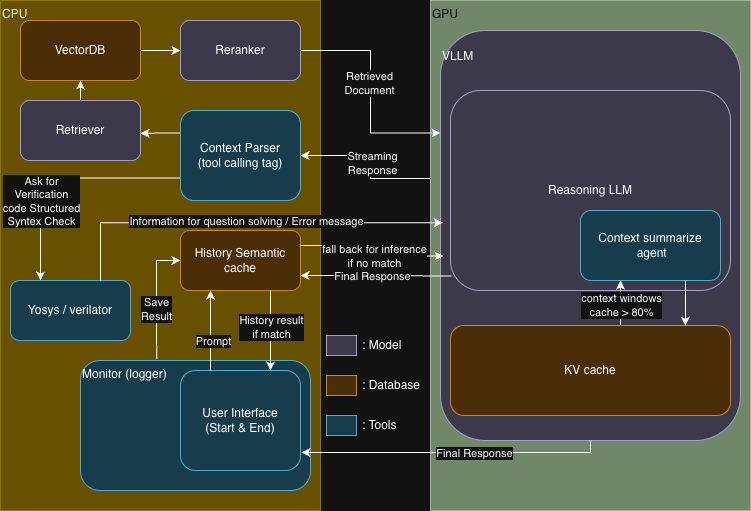
\includegraphics[width=0.95\textwidth]{figures/thesis-Deployment.png}
  \caption[System deployment overview]{Deployment overview: CPU-side
    retrieval, planning, verification, and caching around a GPU-side
    local vLLM inference server.}
  \label{fig:deployment}
\end{figure}

Concretely, this thesis addresses the following problem. Given a
natural-language specification of one Verilog module inside an existing
project --- with the project's other modules provided as source files,
and a hidden-logic testbench fixing the module's exact port contract ---
generate RTL that compiles warning-free with the full project and passes
the testbench, using only local open-weight models
(Figure~\ref{fig:deployment}). Three properties make this hard. The
environment imposes \emph{fatal structural contracts} (re-declaring a
provided module or missing a testbench port kills the sample outright).
The tasks are \emph{heterogeneous} --- thin wrapper modules, algorithmic
datapaths, and thousand-line integrators demand different generation
strategies. And compute is \emph{finite and local}: every planning step,
repair attempt, and sample competes for the same GPU, so a system that
cannot decide where its compute converts is a system that mostly wastes
it.

\section{Contributions}
\label{sec:intro-contributions}

This thesis makes three contributions, each evaluated on the same
60-task benchmark under controlled ablations.

\begin{enumerate}
  \item \textbf{A two-stage agentic IP-reuse pipeline}
    (Chapter~\ref{ch:03}): a planning agent that works the task through
    a suite of IP-reuse tools --- catalog search, candidate inspection
    and scoring, and interface-compatibility verification --- and emits
    a structured reuse plan grounded against a per-task catalog of the
    modules the environment actually provides, followed by a generator
    operating under environment-faithful verification and repair. At
    temperature~0 the pipeline passes 25.0\,\% of tasks against the
    same model's direct 10.0\,\% ($2.5\times$; syntax $2.3\times$),
    with the entire gain concentrated in the reuse-rich processor-core
    family (Section~\ref{sec:results-headline}).
  \item \textbf{A cascade router between generation flows}
    (Chapter~\ref{ch:04}): a two-tier router --- spec-level LLM
    pre-routing plus a plan probe for the uncertain residue --- that
    sends integration-shaped tasks to the pipeline and self-contained
    algorithmic tasks to a cheap direct flow. In its controlled ablation
    it raises solved tasks from 21 to 34 of 60 \emph{while reducing}
    total compute from 213 to 130 hours, and reaches $4\times$ the
    token efficiency per solved task of brute-forcing both flows
    (Section~\ref{sec:results-routing}).
  \item \textbf{Controlled measurements of the supporting machinery}
    (Chapter~\ref{ch:06}): a semantic repair cache that lifts syntax
    monotonically (59.4\,\%$\to$66.9\,\%) while concentrating passing
    samples inside solvable tasks; a repair-budget calibration showing
    both repair phases converge within their first attempts, so compact
    budgets capture nearly all attainable value at a fraction of the
    compute; and a functional repair loop reported as its own
    experimental arm because its feedback signal is the scoring oracle
    --- an accounting line this literature rarely draws.
\end{enumerate}

Throughout, every claim is tied to a controlled comparison, and results
are reported with the same care whether they move the headline metric or
locate exactly where the next gain must come from --- the grounding pass
that made every plan auditable is, we argue, as informative as the
router's $+13$ tasks.

\section{Thesis Organization}
\label{sec:intro-organization}

Chapter~\ref{ch:02} reviews the background and situates the thesis in
four research threads. Chapters~\ref{ch:03} and~\ref{ch:04} present the
pipeline and the router. Chapter~\ref{ch:05} fixes the benchmark,
models, metrics, and the inventory of every experimental run.
Chapter~\ref{ch:06} reports results: the headline comparison, the
ablations, the routing study, a failure taxonomy, and the
benchmark-artifact audit. Chapter~\ref{ch:07} discusses implications,
states threats to validity, and concludes. Appendices collect prompt
templates and per-module result tables.
